\documentclass[12pt]{article}

\usepackage[margin=1in]{geometry}
\usepackage{amsmath, amssymb, amsthm, amsfonts}
\usepackage{tikz}
\usepackage{hyperref}
\usepackage{url}

% ------------------------------------------------------------
% Theorem Environments
% ------------------------------------------------------------
\theoremstyle{plain}
\newtheorem{theorem}{Theorem}[section]
\newtheorem{lemma}[theorem]{Lemma}
\newtheorem{proposition}[theorem]{Proposition}
\newtheorem{corollary}[theorem]{Corollary}

\theoremstyle{definition}
\newtheorem{definition}[theorem]{Definition}
\newtheorem{example}[theorem]{Example}
\newtheorem{remark}[theorem]{Remark}

% ------------------------------------------------------------
% Title and Author
% ------------------------------------------------------------
\title{\textbf{The Universal Linguistic Functor:\\
A Category-Theoretic Framework for Grammar, Semantics, and Variation}}

\author{\textbf{Matthew Long}\\
\textit{Magneton Labs}}
\date{\today}

\begin{document}
\maketitle

\begin{abstract}
We \textbf{propose} a unified category-theoretic framework, called the \emph{Universal Linguistic Functor} (ULF), that integrates syntax, semantics, and cross-linguistic variation. By treating a universal grammar as an \emph{initial object} in the category of grammars, employing \emph{presheaves} to capture language-specific parameters, and using \emph{enriched} and \emph{topos-theoretic} techniques for graded semantics, ULF provides a comprehensive yet flexible approach to linguistic analysis. We outline core definitions, give proof sketches for key theorems, and discuss applications in \textbf{natural language processing} (e.g., structure-preserving translation) and \textbf{cognitive modeling} (e.g., prototype semantics). Our work illustrates how standard categorical tools (functors, adjunctions, presheaves, monads, toposes) can be harnessed to model language in a structurally consistent way.
\end{abstract}

\tableofcontents

\section{Introduction}\label{sec:intro}
A central goal of theoretical linguistics is to balance the \emph{universality} of language---features that all human languages share---with the \emph{variation} that arises across them. The \textbf{Universal Linguistic Functor (ULF)} framework aims to integrate these dimensions by exploiting well-established methods from category theory.

In particular, ULF:
\begin{enumerate}
    \item Treats \emph{universal grammar} as an \textbf{initial object} in the category of grammars (\(\mathbf{Gram}\)).
    \item Models \textbf{cross-linguistic variation} using \textbf{presheaves} over parameter spaces.
    \item Supports \textbf{graded and context-sensitive} semantics by way of \([0,1]\)-enrichment and \emph{topos}-based generalizations.
\end{enumerate}

We build on earlier formulations of ULF, refining the mathematical details, providing expanded proof sketches, and demonstrating the framework's applicability to both \textbf{NLP} tasks and \textbf{cognitive} theories of language comprehension.

\section{Background and Motivation}

\subsection{Why Category Theory?}
Category theory offers a high-level language for describing structures and their relationships via morphisms. It is celebrated for unifying disparate areas of mathematics, theoretical computer science, and even physics. In linguistics, we can cast syntactic derivations and semantic compositions as morphisms in suitable categories.

\begin{definition}[Category]
A \emph{category} \(\mathbf{C}\) consists of:
\begin{itemize}
    \item a class of \emph{objects},
    \item a class of \emph{morphisms} (arrows) between objects,
\end{itemize}
such that morphisms compose associatively, and each object has an identity morphism.
\end{definition}

This viewpoint naturally accommodates the study of how structures (e.g., syntactic trees) map to other structures (e.g., semantic representations) while respecting algebraic constraints.

\subsection{Functors and Adjointness in Linguistics}
\begin{definition}[Functor]
Let \(\mathbf{C}\) and \(\mathbf{D}\) be categories. A \emph{functor} \(F: \mathbf{C} \to \mathbf{D}\) sends each object \(C \in \mathbf{C}\) to an object \(F(C) \in \mathbf{D}\) and each morphism \(f: C \to C'\) to a morphism \(F(f): F(C) \to F(C')\) in a way that preserves identities and composition.
\end{definition}

In linguistics, a functor might map \emph{syntactic} derivations to \emph{semantic} interpretations. Adjoint functors capture deeper correspondences: they can encode dualities between syntax and semantics, or generative and interpretive components of grammar (see \cite{BarkerShan}).

\subsection{Topos Theory and Beyond}
Topos theory generalizes set-theoretic reasoning to an abstract categorical universe. A \emph{Grothendieck topos} provides internal logic, subobject classifiers, and sheaf constructions, potentially modeling intensional or contextual phenomena more flexibly than classical truth-conditional semantics \cite{Awodey}.

\section{The Category of Grammars \texorpdfstring{$\mathbf{Gram}$}{Gram}}
We define \(\mathbf{Gram}\) as the category whose objects are grammars and whose morphisms capture structural homomorphisms between these grammars.

\subsection{Objects: Formal Grammars}
\begin{definition}[Formal Grammar]
A \emph{formal grammar} \(G\) is a 4-tuple
\[
G = (N, \Sigma, P, S),
\]
where:
\begin{itemize}
    \item \(N\) is a set of \emph{nonterminal} symbols,
    \item \(\Sigma\) is a set of \emph{terminal} symbols,
    \item \(P\) is a set of \emph{production rules} (or constraints),
    \item \(S \in N\) is a distinguished \emph{start symbol}.
\end{itemize}
More expressive frameworks (Minimalist Grammars, HPSG, TAGs) can be folded into this scheme by interpreting \(P\) to represent syntactic, morphological, or constraint-based relations.
\end{definition}

\subsection{Morphisms: Grammar Homomorphisms}
\begin{definition}[Grammar Homomorphism]\label{def:grammar-homomorphism}
Let 
\[
G_1 = (N_1, \Sigma_1, P_1, S_1), \quad
G_2 = (N_2, \Sigma_2, P_2, S_2).
\]
A \emph{grammar homomorphism} \(\phi: G_1 \to G_2\) consists of:
\begin{itemize}
    \item A function \(\phi_N: N_1 \to N_2\) preserving start symbols (i.e.\ \(\phi_N(S_1) = S_2\) or its designated counterpart).
    \item A function \(\phi_\Sigma: \Sigma_1 \to \Sigma_2\) that respects terminal correspondences.
    \item A mapping of production rules \(p \in P_1\) to compatible rules in \(P_2\), consistent with \(\phi_N\) and \(\phi_\Sigma\).
\end{itemize}
\end{definition}

\begin{definition}[The Category \(\mathbf{Gram}\)]
\(\mathbf{Gram}\) is the category whose objects are formal grammars and whose morphisms are the grammar homomorphisms of Definition \ref{def:grammar-homomorphism}. Composition is defined by composing the underlying functions \(\phi_N, \phi_\Sigma\) and ensuring production rules remain consistent. The identity morphism on \(G\) is the trivial map that fixes \(N, \Sigma, P, S\).
\end{definition}

\section{Universal Grammar as an Initial Object}
A key tenet of generative linguistics is that a \emph{universal grammar} (UG) underlies all human languages. In the ULF framework, this universal grammar object is initial in \(\mathbf{Gram}\).

\subsection{Definition and Existence}
\begin{definition}[Initial Object]
An object \(I\) in a category \(\mathbf{C}\) is \emph{initial} if for every object \(C\) in \(\mathbf{C}\), there is a \textbf{unique} morphism \(I \to C\).
\end{definition}

\begin{theorem}[Universal Grammar Object]\label{thm:UG}
If a set of universal features and constraints underlies every grammar \(G\) in \(\mathbf{Gram}\), then there exists an \emph{initial object} \(\mathcal{U}\), called the \emph{universal grammar}, such that
\[
\forall G \in \mathbf{Gram}, \quad \exists!\, (\mathcal{U} \to G).
\]
\end{theorem}

\begin{proof}[Sketch]
\textbf{Step 1: Generators.}  
Let \(\mathcal{F}\) be the set of universal features, syntactic categories, morphological principles, etc.

\textbf{Step 2: Relations.}  
Collect universal constraints (e.g., locality, case assignment) into \(\mathcal{R}\). Consider the \emph{free grammar} on \(\mathcal{F}\), then quotient by closure under \(\mathcal{R}\).

\textbf{Step 3: Universal Property.}  
Every grammar \(G\) in \(\mathbf{Gram}\) arises via a unique homomorphism interpreting these universal generators in \(G\). This mirrors free-monoid constructions in universal algebra and establishes \(\mathcal{U}\) as initial.
\end{proof}

\section{Presheaf-Based Language Variation}

\subsection{The Category \texorpdfstring{$\mathbf{Lin}$}{Lin} of Linguistic Contexts}
To handle cross-linguistic differences (e.g.\ head-initial vs.\ head-final, morphological parameters), define a category \(\mathbf{Lin}\) whose objects are parameter configurations and whose morphisms represent transitions among these configurations.

\subsection{Presheaves for Variation}
\begin{definition}[Presheaf]
Given a category \(\mathbf{C}\), a \emph{presheaf} on \(\mathbf{C}\) is a functor
\[
P : \mathbf{C}^{op} \to \mathbf{Set}.
\]
\end{definition}

In our setting, a presheaf
\[
P : \mathbf{Lin}^{op} \to \mathbf{Set}
\]
assigns to each parameter configuration \(L\) a set \(P(L)\) of possible derivations/structures respecting that configuration. The functorial action handles how these sets transform when parameters change along morphisms in \(\mathbf{Lin}\).

\begin{example}[Head Direction: English vs.\ Japanese]
Let \(P\) encode word-order constraints. If \(L_{\mathrm{eng}}\) represents head-initial (Verb-Object) and \(L_{\mathrm{jpn}}\) represents head-final (Object-Verb):
\[
P(L_{\mathrm{eng}})\;=\;\{\text{V+O-structures}\},\quad
P(L_{\mathrm{jpn}})\;=\;\{\text{O+V-structures}\}.
\]
Morphisms between these contexts reflect reordering operations or parameter toggles.
\end{example}

\subsection{Commutative Diagrams and Natural Transformations}
If \(P, Q : \mathbf{Lin}^{op} \to \mathbf{Set}\) are two presheaves representing different linguistic modules (syntax, morphology), a natural transformation \(\alpha : P \to Q\) imposes consistency across modules for each parameter setting.

\begin{theorem}[Presheaf Consistency]\label{thm:PresheafConsistency}
For every morphism \(\sigma: L_2 \to L_1\) in \(\mathbf{Lin}\), a natural transformation \(\alpha : P \to Q\) guarantees the commutativity of
\[
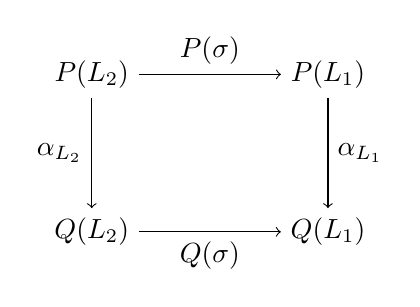
\begin{tikzpicture}[node distance=4em, auto]
  \node (P2) at (0,0) {$P(L_2)$};
  \node (P1) at (3,0) {$P(L_1)$};
  \node (Q2) at (0,-2) {$Q(L_2)$};
  \node (Q1) at (3,-2) {$Q(L_1)$};

  \draw[->] (P2) to node {$P(\sigma)$} (P1);
  \draw[->] (Q2) to node [below] {$Q(\sigma)$} (Q1);
  \draw[->] (P2) to node [left] {$\alpha_{L_2}$} (Q2);
  \draw[->] (P1) to node [right] {$\alpha_{L_1}$} (Q1);
\end{tikzpicture}
\]
Hence, parameter adjustments yield coherent transformations in both presheaves.
\end{theorem}

\begin{proof}[Sketch]
By the definition of naturality, each \(\alpha_{L}\) must commute with the actions of \(P\) and \(Q\) on morphisms in \(\mathbf{Lin}\). This local condition extends to all compositions in \(\mathbf{Lin}\), ensuring global consistency.
\end{proof}

\section{Enriched and Topos-Theoretic Semantics}

\subsection{Enrichment Over \texorpdfstring{$[0,1]$}{[0,1]} for Gradience}
Classical Boolean semantics cannot capture gradable adjectives or partial truth easily. A category \(\mathbf{Sem}\) \emph{enriched} over \(\bigl([0,1], \times, 1\bigr)\) uses real values in \([0,1]\) as hom-objects.

\begin{definition}[Enriched Category Over \texorpdfstring{$[0,1]$}{[0,1]}]
A category \(\mathbf{Sem}\) is \emph{enriched} over \(\bigl([0,1], \times, 1\bigr)\) if, for each pair of objects \(A, B\), \(\mathbf{Sem}(A,B)\) is an element of \([0,1]\). Composition respects the monoidal operation (multiplication) on \([0,1]\).
\end{definition}

Linguistically, a morphism \(A \to B\) in \(\mathbf{Sem}\) can represent \emph{graded} membership or entailment, linking to prototype-theoretic views of categories \cite{Rosch}.

\subsection{Topos-Theoretic Perspective}
A \emph{Grothendieck topos} can serve as a generalized universe of sets and support an internal logic. If \(\mathbf{Lin}\) is viewed as a site (with a Grothendieck topology), then sheaves or presheaves on \(\mathbf{Lin}\) can express intensional contexts (e.g., belief states, possible worlds) more robustly than naive set-based semantics \cite{Awodey}.

\section{Detailed Mathematical Formulations}

\subsection{Universal Grammar in a Monoidal Category}
One can see \(\mathbf{Gram}\) as an object in \(\mathbf{Cat}\), the category of small categories. Further products like \(\mathbf{Gram} \times \mathbf{Lin}\) or \(\mathbf{Gram} \times \mathbf{Sem}\) allow studying how grammars interact with parameter spaces or semantic categories, possibly under a chosen monoidal product \(\otimes\).

\subsection{Monad Structures for Ambiguity}
Monads capture computational effects, including linguistic ambiguity:

\begin{definition}[Monad on \texorpdfstring{$\mathbf{Gram}$}{Gram}]
A \emph{monad} on \(\mathbf{Gram}\) is an endofunctor \(T : \mathbf{Gram} \to \mathbf{Gram}\) equipped with unit \(\eta\) and multiplication \(\mu\) (both natural transformations) such that:
\[
\mu \circ T(\mu) = \mu \circ (\mu)_T, \quad
\mu \circ T(\eta) = \mathrm{id}, \quad
\mu \circ \eta_T = \mathrm{id}.
\]
\end{definition}

Such monads unify multiple possible parses or scope assignments within a single framework, which can be valuable for modeling linguistic phenomena like quantifier scope ambiguity or partial parsing.

\section{Proof Sketches for Key Results}

\subsection{Universal Grammar (Theorem \ref{thm:UG})}
We derived \(\mathcal{U}\) by freely generating from universal features and quotienting out universal constraints, analogous to free objects in universal algebra. Each grammar \(G\) factors uniquely through \(\mathcal{U}\), making \(\mathcal{U}\) an initial object.

\subsection{Presheaf Consistency (Theorem \ref{thm:PresheafConsistency})}
The square-commutativity required by a natural transformation applies at every morphism in \(\mathbf{Lin}\). Because categories are closed under composition, local consistency extends transitively, ensuring global coherence of parameter-based variation.

\section{Applications to NLP}\label{sec:nlp}
We highlight several ways that ULF may enhance \textbf{natural language processing}:

\begin{enumerate}
    \item \textbf{Structure-Preserving Translation:}  
    Use functorial mappings \(\mathbf{Gram}_{\mathrm{src}} \to \mathbf{Gram}_{\mathrm{tgt}}\) to align morphological and syntactic structures more transparently than purely statistical approaches.

    \item \textbf{Parameter Discovery:}  
    Model morphological/syntactic parameters as objects in \(\mathbf{Lin}\). Presheaf analysis guides unsupervised or semi-supervised \emph{parameter induction}, supporting cross-linguistic typological learning.

    \item \textbf{ULF-Based Parsers:}  
    Implement parsing algorithms where states correspond to grammar objects, and transitions are grammar homomorphisms. This approach can constrain search spaces for more robust, explainable parsing.

    \item \textbf{Hybrid Symbolic--Neural Models:}  
    Integrate deep learning with a category-theoretic backbone, combining neural efficiency with symbolic compositional constraints \cite{KleinManning}.
\end{enumerate}

\section{Cognitive Modeling}\label{sec:cog}
ULF also opens up avenues for \textbf{cognitive} theories:

\begin{enumerate}
    \item \textbf{Prototype Semantics:}  
    By enriching over \(\bigl([0,1], \times, 1\bigr)\), ULF handles gradual category membership (e.g., \emph{robin} is a more prototypical \emph{bird} than \emph{penguin}), reflecting \cite{Rosch}.

    \item \textbf{Neural Correlates of Gradience:}  
    Empirically test whether neural signals (fMRI, EEG) mirror the graded truth values predicted by enriched categories.

    \item \textbf{Monadic Ambiguity Resolution:}  
    Human parsing often entertains multiple interpretations (garden-path sentences) before settling on a single parse. Monads naturally capture such branching and subsequent resolution.

    \item \textbf{Context Evolution in Toposes:}  
    Model dynamic semantics via internal logic in a topos, where discourse updates correspond to morphisms. This connects formal semantics with psychological models of context tracking.
\end{enumerate}

\section{Summary of the Formula}
\label{sec:summary_formula}
The \emph{universal linguistic functor} $U$ describes how linguistic objects are mapped to semantic representations:

\[
U : \mathcal{L} \;\xrightarrow{\;\mathcal{H}\;} \mathbf{Ch} \;\xrightarrow{\;\Phi\;} \mathcal{S},
\]
where:
\begin{itemize}
    \item $\mathcal{L}$ is a \textbf{linguistic category} of syntactic/phonological objects,
    \item $\mathbf{Ch}$ is a category (e.g., chain complexes) encoding structural adjacency,
    \item $\mathcal{H}\colon \mathcal{L} \to \mathbf{Ch}$ captures structural relations,
    \item $\Phi\colon \mathbf{Ch} \to \mathcal{S}$ interprets those chain complexes in a \textbf{semantic category} $\mathcal{S}$.
\end{itemize}
Composing $\mathcal{H}$ and $\Phi$ yields a single pipeline from linguistic form to semantic content.

\section{Future Directions and Open Problems}

\subsection{Homotopy Type Theory (HoTT)}
HoTT may extend ULF by treating syntactic transformations (e.g., passivization, wh-movement) as homotopies in higher categories, identifying paraphrase relations with higher equivalences.

\subsection{ULF Benchmarks for Generalization}
To test compositional generalization, propose \textbf{ULF-based benchmarks} that highlight whether models can truly interpret grammar homomorphisms and parameter toggles, akin to SCAN-style tasks.

\subsection{Computational Complexity}
Despite the elegance of category-theoretic formulations, large-scale parsing or semantic inference must remain computationally feasible. Developing efficient (polynomial-time) algorithms that leverage ULF constraints is a pressing challenge.

\subsection{Extended Topos Constructions}
Dialects, code-switching, or register shifts might require more intricate sheaf constructions on a site representing sociolinguistic contexts, bridging macrosociological data with advanced categorical methods.

\section{Conclusion}
By positing an \emph{initial universal grammar object}, modeling cross-linguistic parameters with \emph{presheaves}, and embedding enriched/topos-theoretic semantics, the \textbf{Universal Linguistic Functor} framework offers a mathematically coherent approach unifying syntax, semantics, and linguistic variation. We also provided \textbf{recommendations} for leveraging these ideas in practical NLP systems and cognitive modeling experiments. Ongoing work explores extensions into \emph{Homotopy Type Theory} and computational complexity, reinforcing ULF’s potential to unify theoretical linguistics, computational methods, and empirical research in one powerful category-theoretic paradigm.

\subsection*{Acknowledgments}
We gratefully acknowledge colleagues in mathematics, linguistics, and computer science for their formative feedback on these ideas. Any remaining errors belong to the authors.

% ------------------------------------------------------------
% References
% ------------------------------------------------------------
\begin{thebibliography}{99}

\bibitem{Awodey}
Awodey, S. (2010). \textit{Category Theory} (2nd ed.). Oxford University Press.

\bibitem{BarkerShan}
Barker, C., \& Shan, C. (2014). \textit{Continuations and Natural Language}. Oxford University Press.

\bibitem{KleinManning}
Klein, D., \& Manning, C. D. (2003). \textit{Accurate Unlexicalized Parsing}. In \textit{Proceedings of the 41st Annual Meeting of the ACL}.

\bibitem{Rosch}
Rosch, E. (1978). Principles of Categorization. In E. Rosch \& B. B. Lloyd (Eds.), 
\textit{Cognition and Categorization}, pp. 27--48. Lawrence Erlbaum.

\end{thebibliography}

\end{document}
